\documentclass[tikz, preview]{standalone}

\usepackage{amsfonts, amsthm, amssymb, amsmath, stmaryrd, etoolbox}
\usepackage{tikz}
\usetikzlibrary{matrix,arrows}

\begin{document}
	\[
	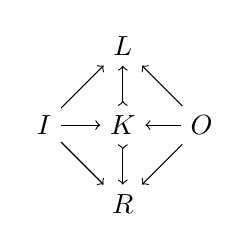
\begin{tikzpicture}
	\node (I) at (-1,0) {$I$};
	\node (O) at (1,0) {$O$};
	\node (L) at (0,1) {$L$};
	\node (K) at (0,0) {$K$};
	\node (R) at (0,-1) {$R$};
	%
	\draw [->] (I) edge (L);
	\draw [->] (I) edge (K);
	\draw [->] (I) edge (R);
	\draw [->] (O) edge (L);
	\draw [->] (O) edge (K);
	\draw [->] (O) edge (R);
	\draw [>->] (K) edge (L);
	\draw [>->] (K) edge (R);
	\end{tikzpicture}
	\]
\end{document}
